%(Mercado, costos, ciclo de vida, %VAN, TIR)
Para poder estudiar la viabilidad financiera de todo emprendimiento es necesario hacer un balance cuidadoso de los diferentes costos en los que se va a incurrir. Se debe analizar cuales serán la fuentes de ingresos que hagan del modelo de negocio planteado un negocio sostenible en el tiempo. 
En este caso en particular estamos analizando el caso de un proyecto único. Sin embargo, no se desea descartar la posibilidad de realizar más unidades en el futuro por fuera del marco del proyecto. Es por esto que presentamos aquí debajo el modelo de negocios planteado para referencia futura. 
\Subsubsection{Modelo de Negocios}

Este diseño se trata de un proyecto único, con posibilidad de realizar hasta \unidadespostfin unidades adicionales posteriores a su finalización. Para dar una visión global se planteo el siguiente modelo de Canvas:
 

\begin{figure}[H]
	\centering
	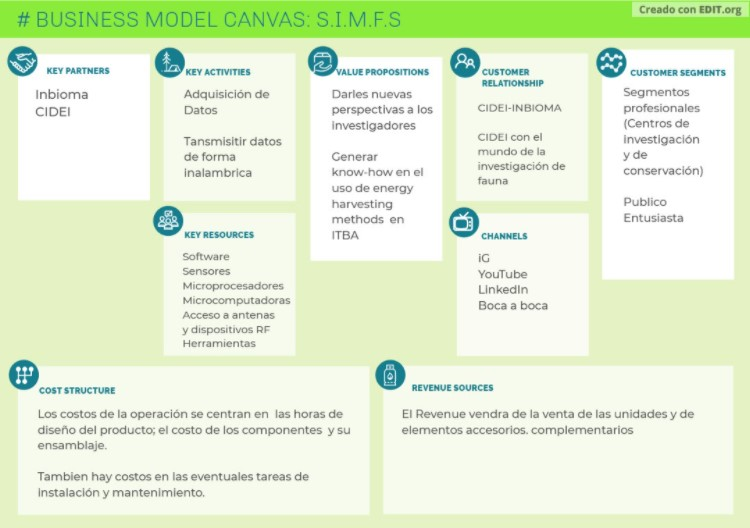
\includegraphics[scale=0.7]{../Factibilidad/ImagenesFactibilidad/ModeloDeCanvas}
	\caption{Modelo de negocio.}
	\label{fig:modelodecanvas}
\end{figure}



\Subsubsection{Investigación y Desarrollo}
Este proyecto contiene una gran componente de diseño. Según lo establecido en la programación del proyecto, el tiempo invertido de diseño esta estimado en 5472 horas. %todas las horas hasta "integracion a nivel modulos" sin incluir
Una vez completada la etapa de diseño el equipo se aboca a la implementación del primer prototipo, es decir a la integración del hardware a utilizar y el desarrollo del software que controla al nido que permite la interacción con el mismo. 

Realizando la estimación sobre un sueldo de $30 \ \frac{USD}{hora}$ y multiplicándolo por la cantidad de horas de ingeniería esperada por persona se obtiene un total de: $$Costo \ mano \ de \ obra = 7100 \ hora \ \cdot 30 \ \frac{USD}{hora} = 213.000,00 \ USD$$


\Subsubsection{Gastos fijos por unidad}

Los gastos principales considerados son USD$259.09$. %Para la compra de los componentes, se suman los costos estimados previamente, más el resto de los componentes misceláneos (resistores, capacitores, etc.) para el diseño de los circuitos involucrados.
%Se estima de este modo un costo de componentes de \TBD USD, a contabilizar una única vez por unidad.

Se presenta el valor de los insumos de hardware y de montaje:
\begin{table}[H]
\centering
\begin{tabular}{|c|c|}
\hline
\textbf{Item}                                                         & \textbf{Precio [USD]}				  \\ \hline
Sensor humedad-temperatura 											  & 4.9                                   \\ \hline
Sensor luminosidad                                                    & $1.54    $                              \\ \hline
M\'odulo RTC                                                     & $2.33$                                  \\ \hline
Cámara                                                                & $20$                                    \\ \hline
SDI 32GBy                                                             & $32$                                    \\ \hline
R-Pi 3B
 & $25.5$                                  \\ \hline
Batería                                                               & $86  $                 				  \\ \hline
Panel solar                                                           & $30$ 				  \\ \hline
MPPT                                                                  & $18$                                    \\ \hline
Encapsulado                                                           & $16$                                    \\ \hline
Módulo Bluetooth 5.0                                                           & $3.82 $                                   \\ \hline
Montaje                                                               & $31$                                    \\ \hline
Extras
& $15$									\\ \hline
\textbf{Total}
&\textbf{$259.09$}
\end{tabular}
\caption{Valores de insumos.}
\end{table}


\Subsubsection{Reserva de Contingencia}
Dado que este proyecto cuenta con un alto grado de investigación es necesario contar con un cierto margen de seguridad en caso de que ocurra un cambio de planes necesario para alcanzar el objetivo del proyecto. Es por eso que se decidió incluir en nuestro análisis un adicional del 5\% sobre el costo total del proyecto. Esta suma sera devuelta al cliente en caso de no necesitarla.

La reserva de contingencia se ubicara en  USD 11.000
\Subsubsection{Escenario de Escala}
Se contempla que en el caso de que la producción sea de \unidadespostfin unidades será posible conseguir los insumos necesarios para el ensamblado de las unidades a precio de venta al por mayor.
